%! Author = drakanoy
%! Date = 10.09.2024

% Preamble
\documentclass[12pt]{article}

% Packages
\usepackage[utf8]{inputenc}
\usepackage[T2A]{fontenc}
\usepackage[english, russian]{babel}
\usepackage[a4paper, includefoot, left=1.5cm, right=1.5cm, top=1cm, bottom=1.5cm, headsep=1cm, footskip=1cm]{geometry}
\usepackage{makecell}
\usepackage{amsmath}
\usepackage{graphicx}
\usepackage{enumitem}
\usepackage{svg}
\usepackage{multirow}
\usepackage{hyperref}
\usepackage{mathtools}
\usepackage{amssymb}
\usepackage{textcomp}

% Document
\begin{document}
\begin{large}
\begin{center}
\LARGE \textbf{Домашняя работа}
\par
\LARGE \textbf{Кононов Александр Михайлович}
\par
    \textbf{16.12.2024}
\end{center}
\par Условие:
\par
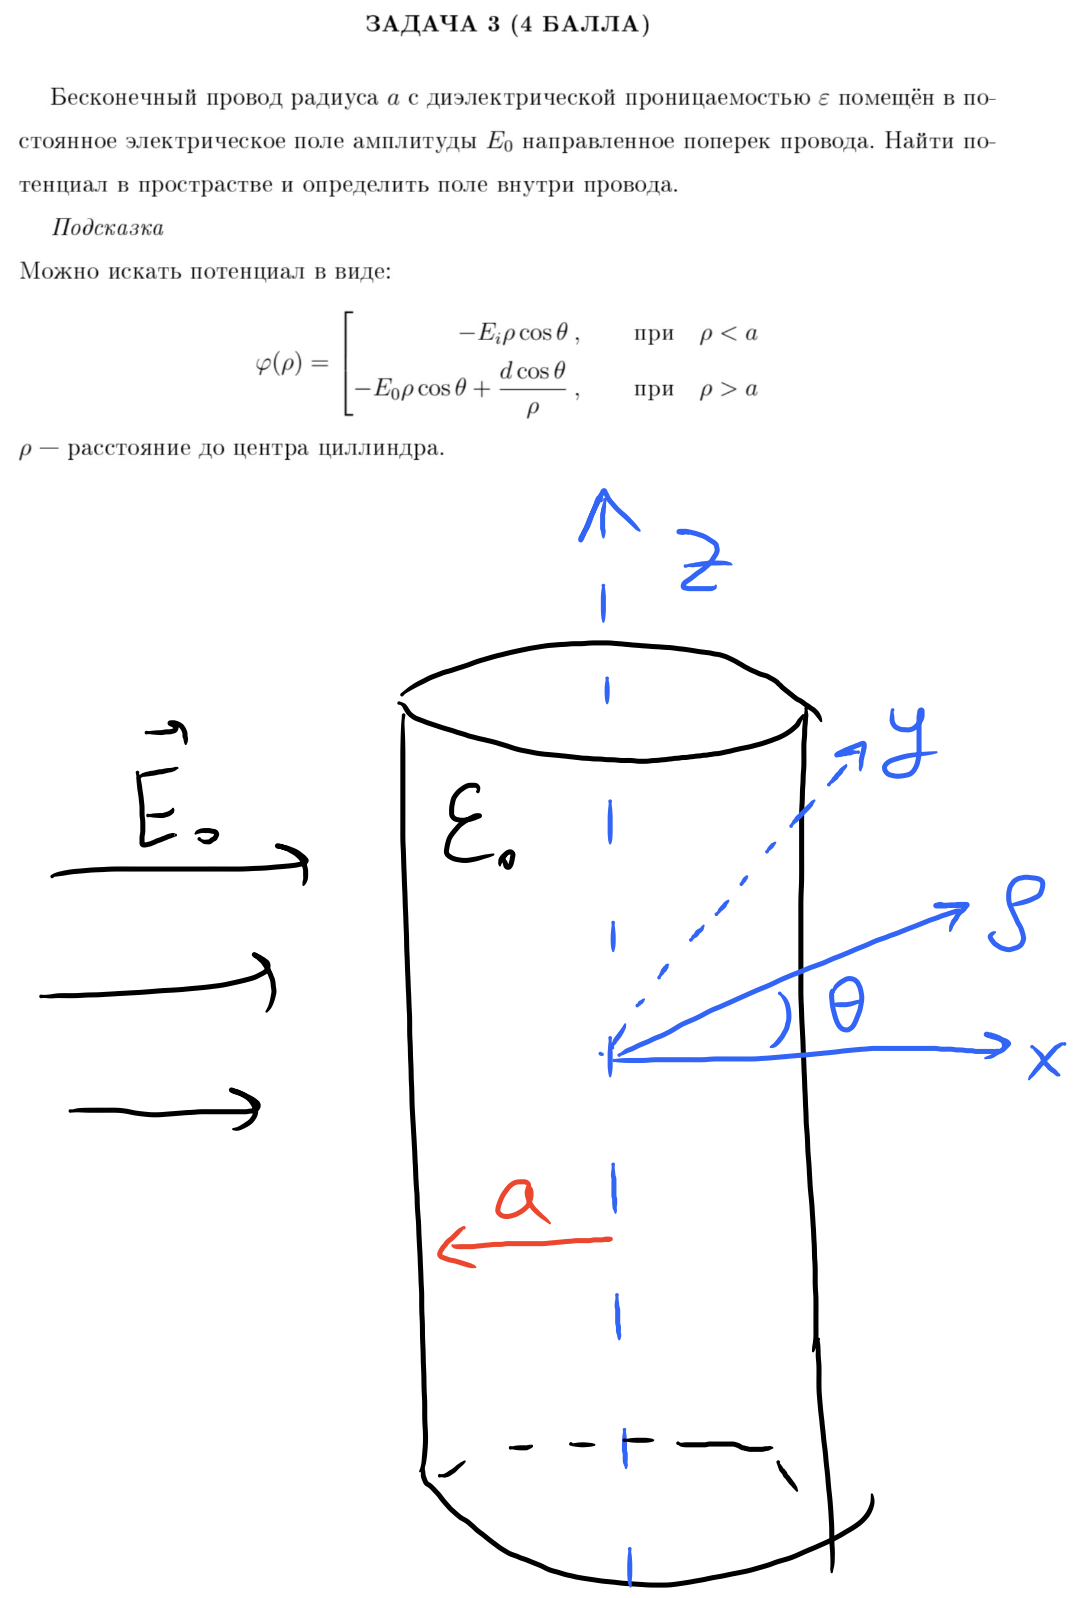
\includegraphics[width=1\textwidth]{photo.png}
%\begin{center}
%\underline{Рисунок 1}:
%\end{center}
\par Решение:
\par
\par
%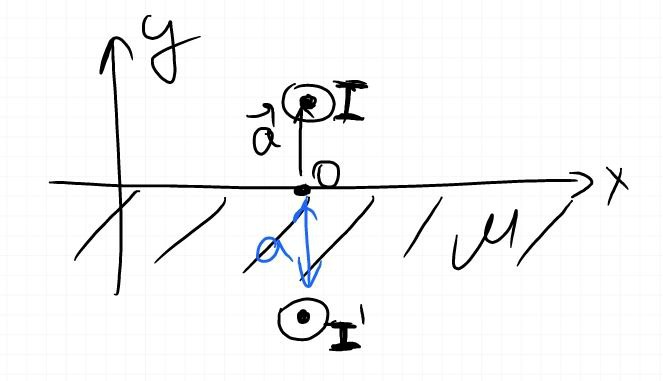
\includegraphics[width=1\textwidth]{photo_1.jpg}
%\par
\begin{center}
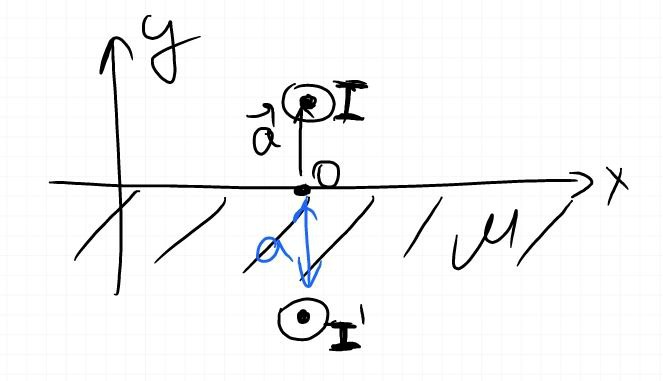
\includegraphics[width=0.4\textwidth]{photo_1.jpg}
\end{center}
\begin{eqnarray*}
    \begin{cases}
        \Delta \overrightarrow{E} + \frac{\varepsilon \omega^2}{c^2} \overrightarrow{E} = 0 ; 0 < z < b \\
        \Delta \overrightarrow{E} + \frac{\omega^2}{c^2} \overrightarrow{E} = 0 ; b < z < a
    \end{cases}
\end{eqnarray*}
\par Так как у нас $E_y = E_z = 0$, то
\begin{eqnarray*}
    \begin{cases}
        \Delta E_x + \frac{\varepsilon \omega^2}{c^2} E_x = 0 ; \,\, 0 < z < b \\
        \Delta E_x + \frac{\omega^2}{c^2} E_x = 0 ; \,\, b < z < a
    \end{cases}
\end{eqnarray*}
\par Граничные условия:
\[
    \varepsilon_1 E_{1n} = \varepsilon_2 E_{2n} ; \,\,\, E_{1\tau} = E_{2\tau}
\]
\par при $y = 0, a$, $z = 0, a$:
\[
    E_x = 0
\]
\par при $x = 0, a$:
\[
    E_x' = 0
\]
\par при $z = b$:
\[
    E_x(b-0) = E_x(b+0) ; \,\,\, E_x'(b-0) = E_x'(b+0)
\]
\[
    E_x = X(x) \cdot Y(y) \cdot Z(z)
\]
\par Магия матфизики:
\[
    X = A \cos(k_x \cdot x) ; \,\, k_x = \frac{\pi n}{a} \,\, n \in \mathbb{Z}
\]
\[
    Y = B \sin(k_y \cdot y) ; \,\, k_y = \frac{\pi m}{a} \,\, m \in \mathbb{Z}
\]
\par $\Rightarrow$ уравнение на $Z$:
\begin{eqnarray*}
    \begin{cases}
        \frac{Z''}{Z} = -\frac{\varepsilon \omega^2}{c^2} + k_x^2 + k_y^2 \\
        \frac{Z''}{Z} = -\frac{\omega^2}{c^2} + k_x^2 + k_y^2
    \end{cases}
\end{eqnarray*}
\begin{eqnarray*}
    \begin{cases}
        Z'' \left( \frac{\varepsilon \omega^2}{c^2} - k_x^2 - k_y^2 \right) Z = 0 \\
        Z'' \left( \frac{\omega^2}{c^2} - k_x^2 - k_y^2 \right) Z = 0
    \end{cases}
\end{eqnarray*}
\par при $0 < z < b$:
\[
    Z_1 = A \sin\left(\sqrt{\frac{\varepsilon \omega^2}{c^2} - k_x^2 - k_y^2} z\right)
\]
\par при $b < z < a$:
\[
    Z_{2} = B \sin\left(\sqrt{\frac{ \omega^2}{c^2} - k_x^2 - k_y^2} \left(z-a\right)\right)
\]
\par теперь $z = b$:
\begin{eqnarray*}
    \begin{cases}
        A \sin\left(\sqrt{\frac{\varepsilon \omega^2}{c^2} - k_x^2 - k_y^2} b\right) = B \sin\left(\sqrt{\frac{ \omega^2}{c^2} - k_x^2 - k_y^2} \left(b-a\right)\right) \\
        A \sqrt{\frac{\varepsilon \omega^2}{c^2} - k_x^2 - k_y^2} \cos\left(\sqrt{\frac{\varepsilon \omega^2}{c^2} - k_x^2 - k_y^2} b\right) = B \sqrt{\frac{\omega^2}{c^2} - k_x^2 - k_y^2} \cos\left(\sqrt{\frac{\omega^2}{c^2} - k_x^2 - k_y^2} \left(b-a\right)\right)
    \end{cases}
\end{eqnarray*}
\par $det = 0$:
\[
    \frac{\tan\left( \sqrt{\frac{\varepsilon \omega^2}{c^2} - k_x^2 - k_y^2} b\right)}{ \sqrt{\frac{\varepsilon \omega^2}{c^2} - k_x^2 - k_y^2}} = \frac{\tan\left( \sqrt{\frac{ \omega^2}{c^2} - k_x^2 - k_y^2} \left(b-a\right)\right)}{ \sqrt{\frac{ \omega^2}{c^2} - k_x^2 - k_y^2}}
\]
\par Пусть $\varepsilon = 1$:
\[
    \Rightarrow \tan\left( \sqrt{\frac{\omega^2}{c^2} - k_x^2 - k_y^2} b\right) = \tan\left( \sqrt{\frac{ \omega^2}{c^2} - k_x^2 - k_y^2} \left(b-a\right)\right)
\]
\[
    \Rightarrow \sqrt{\frac{\omega^2}{c^2} - k_x^2 - k_y^2} b  = \sqrt{\frac{ \omega^2}{c^2} - k_x^2 - k_y^2} \left(b-a\right) + \pi p ; \,\, p \in \mathbb{Z}
\]
\[
    \frac{\omega^2}{c^2} - k_x^2 - k_y^2 = \frac{\pi^2p^2}{a^2}
\]
\[
    \frac{\omega^2}{c^2} = k_x^2 + k_y^2 + \frac{\pi^2p^2}{a^2}
\]
\[
    \frac{\omega^2}{c^2} = \frac{\pi^2n^2}{a^2} + \frac{\pi^2m^2}{a^2} + \frac{\pi^2p^2}{a^2} ; \,\, n, m, p \in \mathbb{Z}
\]
\[
    \omega = \frac{c \pi}{a}\sqrt{n^2 + m^2+ p^2} ; \,\, n, m, p \in \mathbb{Z}
\]
\par Ответ:
\[
    \frac{\tan\left( \sqrt{\frac{\varepsilon \omega^2}{c^2} - k_x^2 - k_y^2} b\right)}{ \sqrt{\frac{\varepsilon \omega^2}{c^2} - k_x^2 - k_y^2}} = \frac{\tan\left( \sqrt{\frac{ \omega^2}{c^2} - k_x^2 - k_y^2} \left(b-a\right)\right)}{ \sqrt{\frac{ \omega^2}{c^2} - k_x^2 - k_y^2}}
\]
\[
    \omega = \frac{c \pi}{a}\sqrt{n^2 + m^2+ p^2} ; \,\, n, m, p \in \mathbb{Z}
\]
\par
\par
\end{large}
\end{document}
